\section{Analysis}
\label{Analysis}

\subsection{Cancelation of Detector Efficiencies, Drifts, and Geometric Phase Space}
\label{subsec:SPDPCancelation}
The efficiency and acceptance of the neutron detection system varies greatly over its opening angle range of 20$^{\circ}$ to 180$^{\circ}$, as illustrated in Fig.~\ref{fig:DetAcceptance}.
This is both due to the neutron detection system's non-spherical symmetry and to varying efficiency as a function of particle position on the detector.
In order to give a result that is sensitive to angular correlations and is not sensitive to detector efficiencies and experimental drifts in PMT voltage, accelerator current, etc. , angular correlation is determined by dividing a correlated neutron distribution by an uncorrelated neutron distribution:
\begin{equation}
\label{eq:angularCorr}
\text{angular correlation }  = \frac{nn_{\text{corr}}(\theta)}{nn_{\text{uncorr}}(\theta)},
\end{equation}
where $nn_{\text{corr}}(\theta)$ is the accidental-coincidence subtracted opening angle distribution, the determination of which is described in section~\ref{Reconstruction of Accidental Coincidence}, and where $nn_{\text{uncorr}}(\theta)$\footnote{While this notation implies that coincident events are only due to neutrons, about 3\% of total  $nn_{\text{corr}}(\theta)$ events are not due to neutrons. This was determined by comparing data from a non-neutron producing Al target to that from a $^{238}$U target (see Fig.~\ref{fig:Noise})} is the uncorrelated neutron distribution, which is produced by the pairing of neutron events that occurred during different pulses.
\begin{figure}[h]
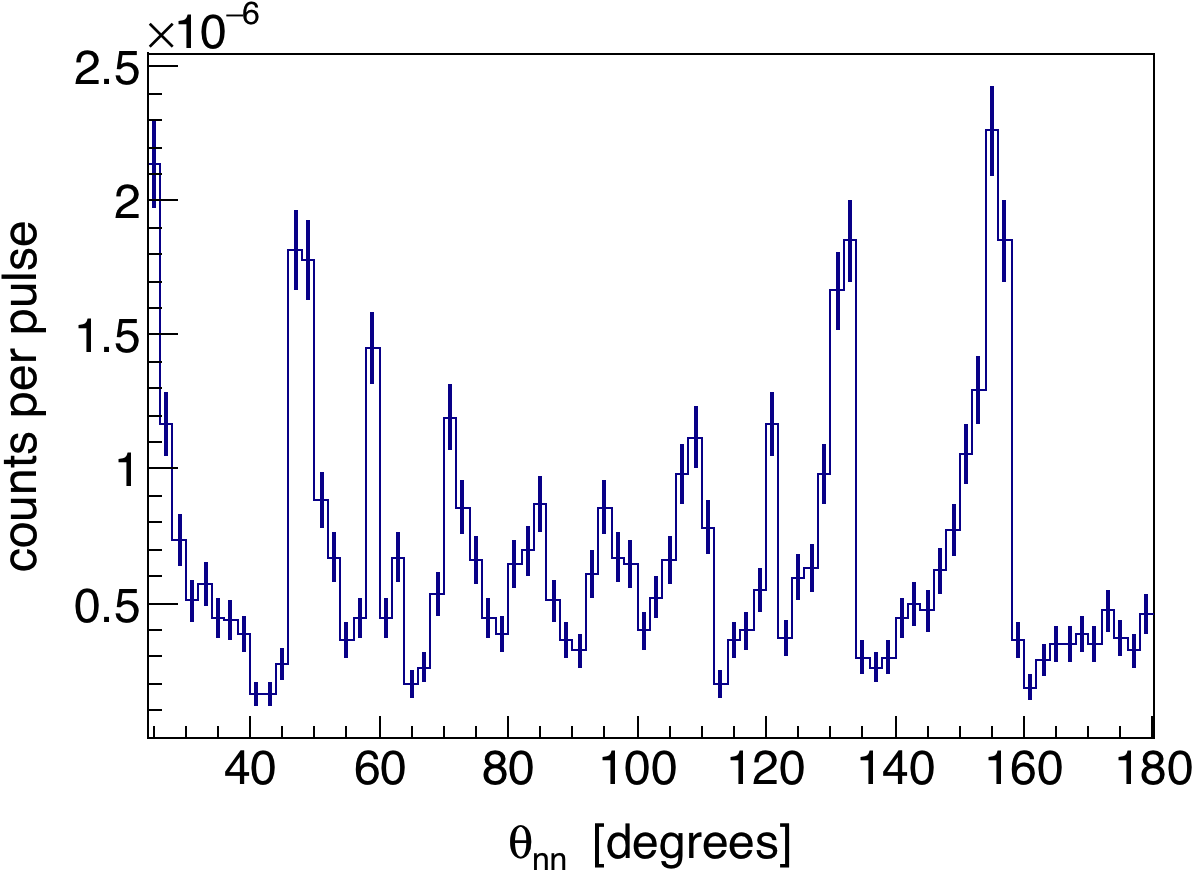
\includegraphics[width=0.9\textwidth]{Content/Methods/DetAcceptance.png}
\caption{Raw n-n opening angle measurement from the photofission of $^{238}$U. 
This distribution is highly influenced by the detection system's geometry and efficiency.
}
\label{fig:DetAcceptance}
\end{figure}

The construction of $nn_{\text{uncorr}}(\theta)$ is achieved by examining pulses in pairs of two under the requirement that both pulses occurred within 0.2 seconds of each other, which makes it very likely that they occurred under the same experimental conditions.
For each pulse-pair that has two neutron events in both pulses, all possible pairs of uncorrelated neutrons are formed (a total of 4 in this case), and the opening angle of each uncorrelated neutron-neutron (n-n) pair is calculated.
The reason for considering only pulse-pairs with two events in each pulse is to increase the percentage of pulse-pairs comprising neutrons from fission as opposed to neutrons from $(\gamma,n)$.
This matters because the detection of multiple neutrons from $(\gamma,n)$ are completely removed from $nn_{\text{corr}}(\theta)$, the numerator in Eq.~\ref{eq:angularCorr}, by the subtraction of accidental coincidences, but in order to effectively minimize the dependence of the result on detector geometry/efficiency, the numerator and denominator of Eq.~\ref{eq:angularCorr} must comprise neutron pairs with a similar energy distribution.

Because $nn_{\text{corr}}(\theta)$ is comprised of correlated n-n pairs, it is important to consider how the energies of both neutrons in n-n pairs vary together, or, in other words, the joint neutron energy distribution.
For this reason, Fig.~\ref{fig:erg_distributions} plots the distributions of two binary operations applied to the energies of n-n pairs: the mean,~$0.5(E_{1} + E_{2})$, and absolute difference, ~$|E_1 - E_2|.
The following three sets of n-n pairs are plotted: correlated n-n pairs (~$nn_{\text{corr}}(\theta)$~), different pulse n-n pairs using only pulses that had two neutron events (~$nn_{\text{uncorr}}(\theta)$~), and different pulse n-n pairs with no restriction on the number of events in a given pulse.
From Fig.~\ref{fig:erg_distributions}, it can be concluded that the joint neutron energy distributions of n-n pairs from $nn_{\text{uncorr}}(\theta)$ and $nn_{\text{corr}}(\theta)$ are very similar.

\begin{figure}[]
\centering
    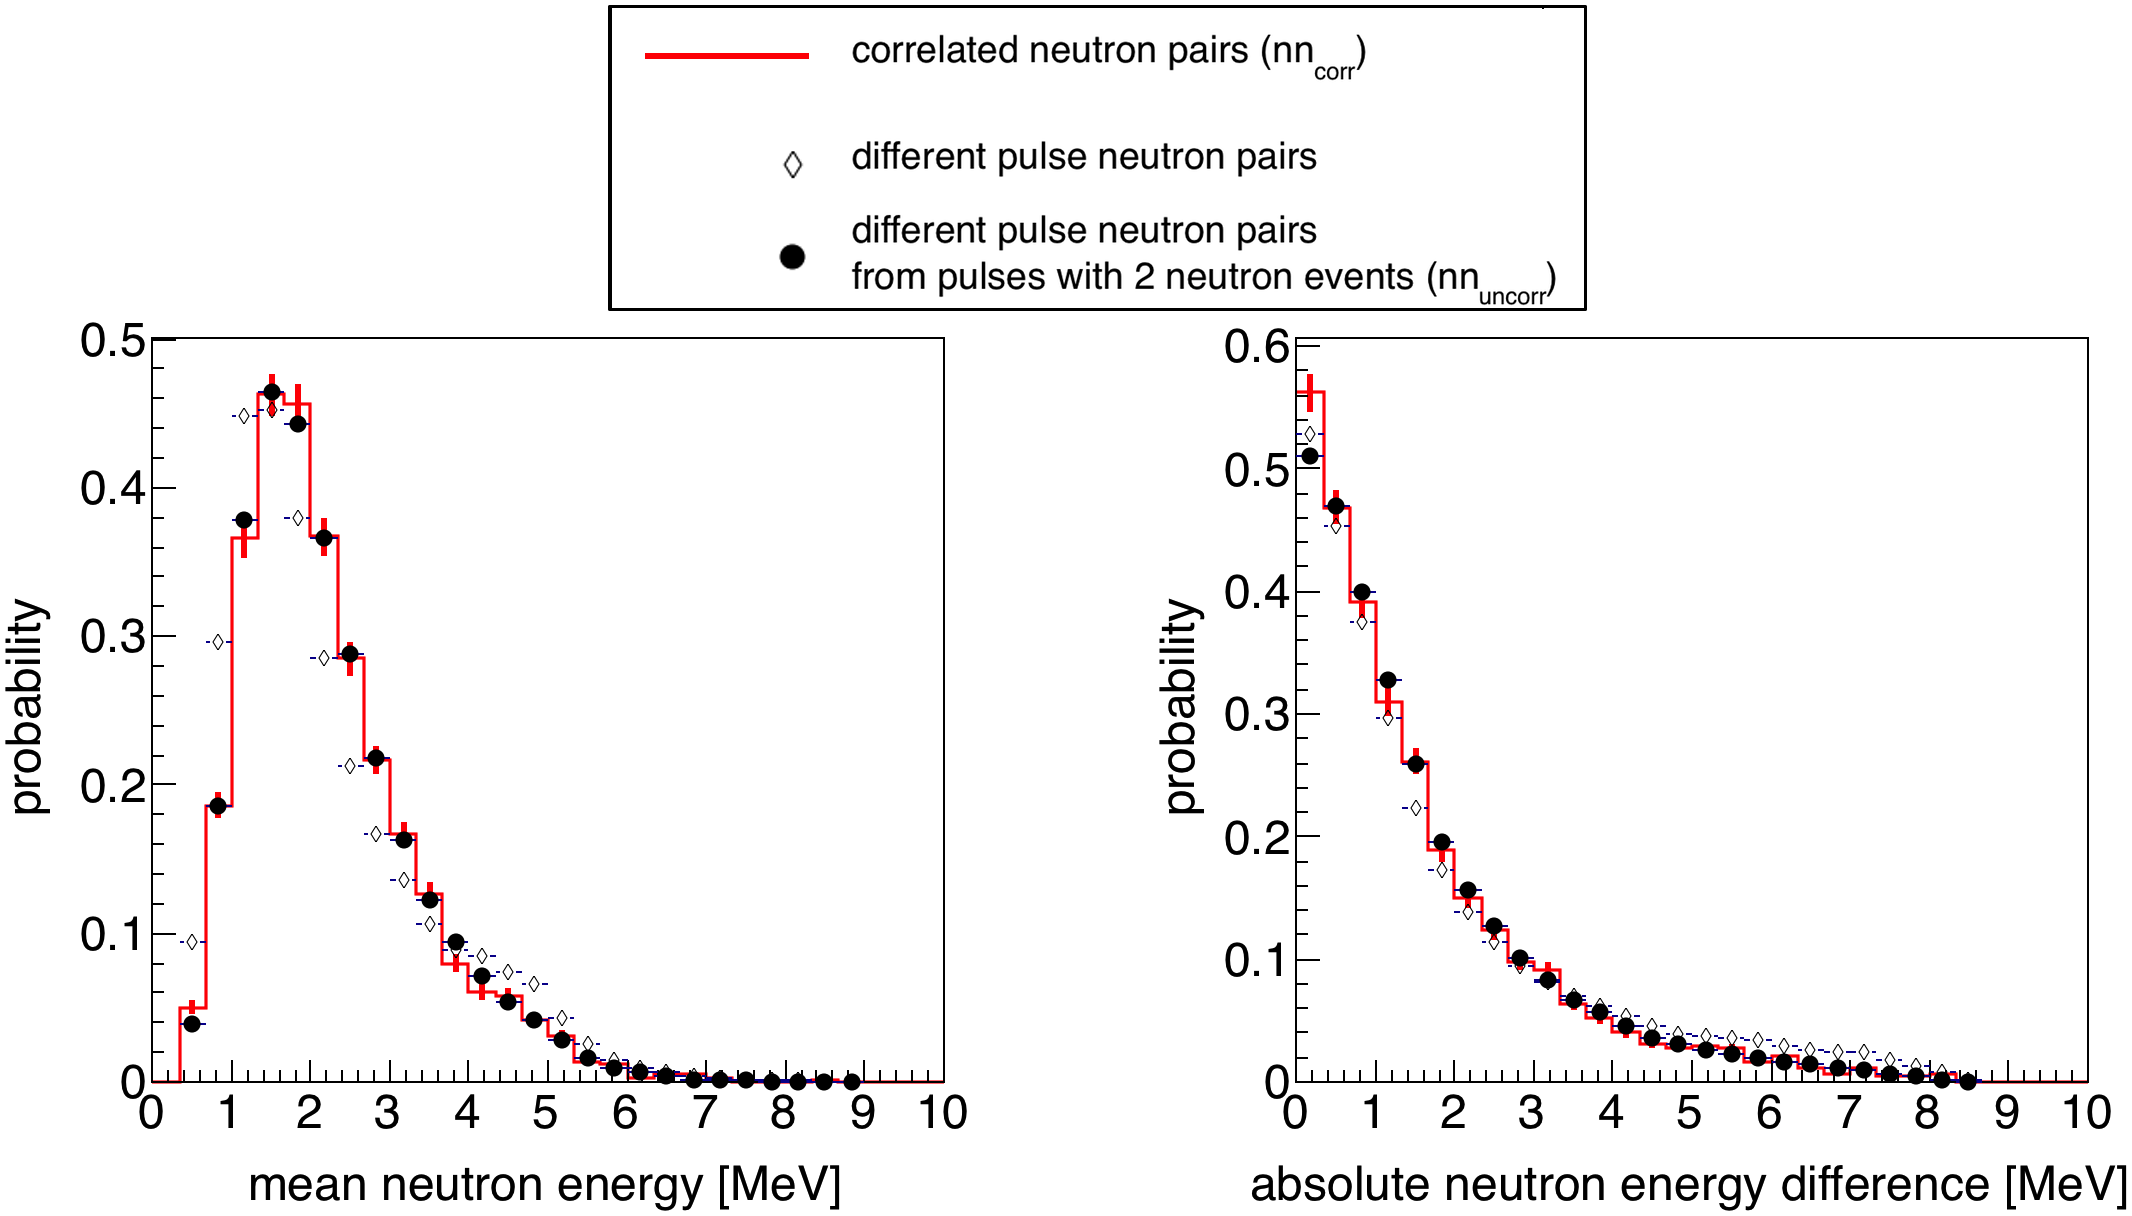
\includegraphics[width=0.99\textwidth]{Content/Methods/erg_dist(thesis).png}
    \caption{
    The energy distribution of n-n pairs from $nn_{\text{corr}}(\theta)$ must be similar to those from $nn_{\text{uncorr}}$ in order for detector efficiency to cancel in Eq.~\ref{eq:angularCorr}.
        For this reason, when determining the uncorrelated neutron distribution by pairing neutron events from different pulses, only pulses which had two neutron events are used.
    This creates a $nn_{\text{uncorr}}$ distribution that uses a higher portion of neutrons from fission relative to neutrons from ($\gamma, 1n$), leading to an energy distribution that's more similar to that of the n-n pairs comprising $nn_{\text{corr}}(\theta)$.
    }
    \label{fig:erg_distributions}
\end{figure}

Figure~\ref{fig:SPDPNormalization}(a) shows the measured $nn_{\text{corr}}(\theta)$ yield distribution of neutrons from the photofission of $^{238}$U.
The structure seen here is reflective of the underlying n-n angular correlations as well as the geometric acceptance and efficiencies of the neutron detectors.
Figure~\ref{fig:SPDPNormalization}(b) reveals how a clear picture of n-n correlations emerges when taking the ratio between $nn_{\text{corr}}(\theta)$ and $nn_{\text{uncorr}}(\theta)$.
\begin{figure}[]
\centering
    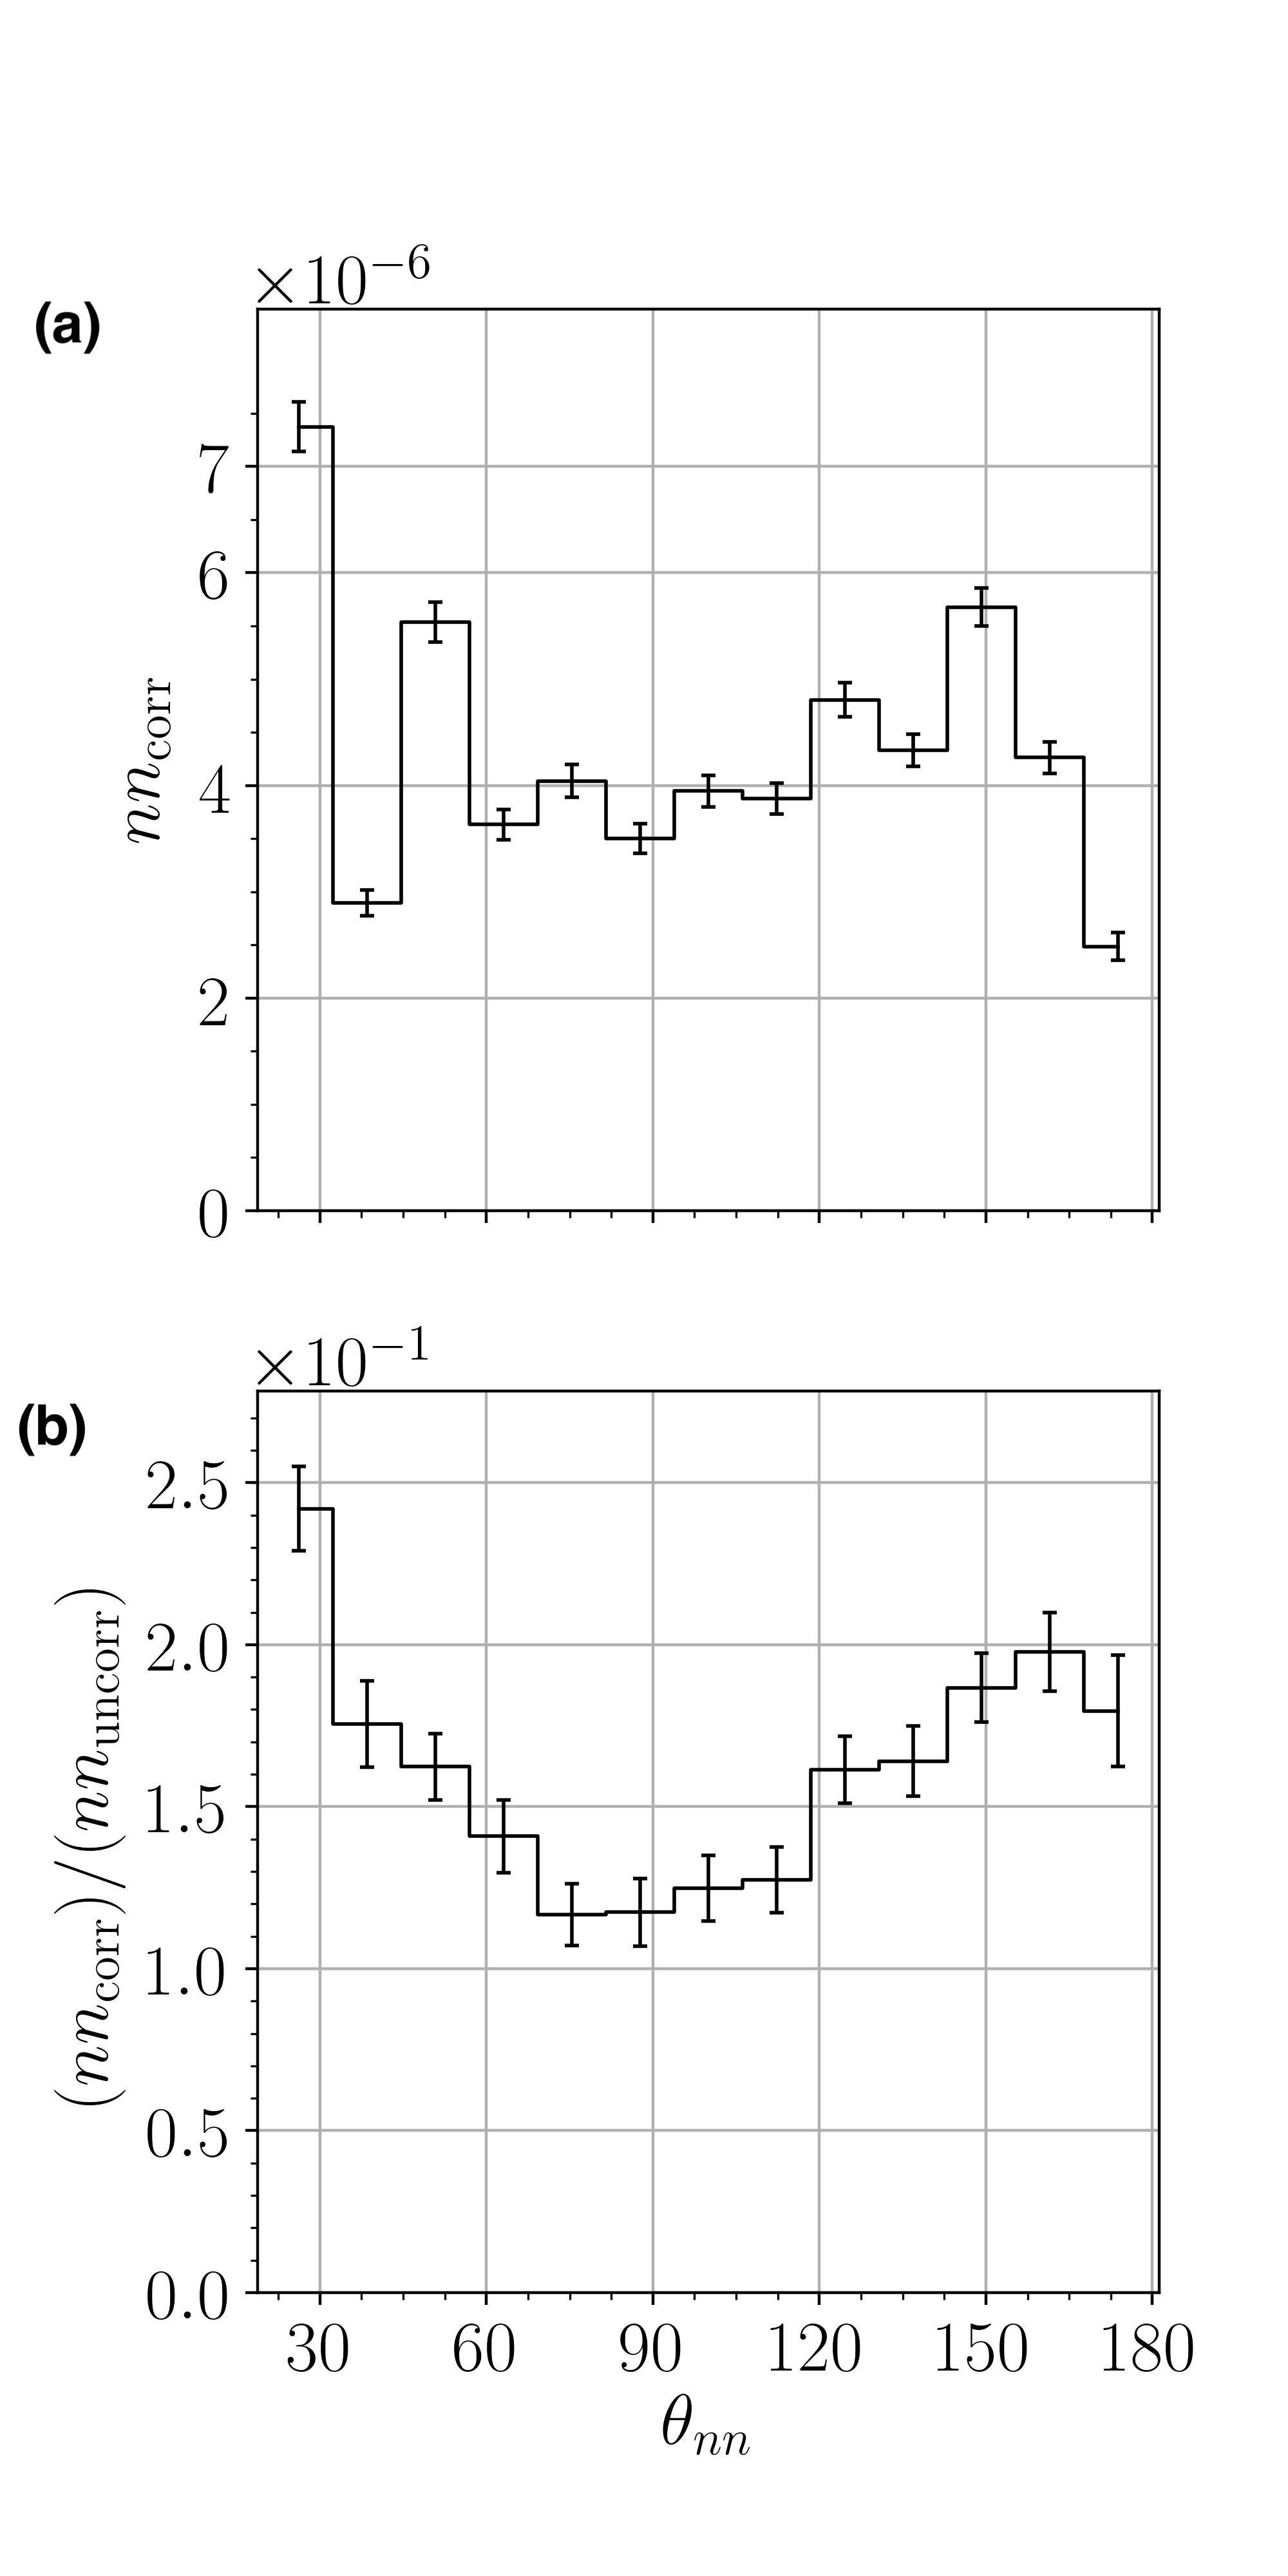
\includegraphics[width=0.7\textwidth]{Content/Methods/SPDPNormalization.png}
    \caption{(a) n-n opening angle distribution from the photofission of $^{238}$U before normalization, and, (b) after normalizing to the distribution of uncorrelated n-n events from different pulses.
    All measured neutrons have an energy greater than 0.4 MeV.}
    \label{fig:SPDPNormalization}
\end{figure}

The n-n opening angle distribution of accidental neutron coincidences from the photo-disintegration of D$_{2}$O is expected to be flat.
A cylindrical bottle with a height of 4.5~cm and a radius of 1~cm was filled with heavy water 
(D$_{2}$O) and subject to the bremsstrahlung photon beam, producing neutron coincidences at a rate of 1.4$\times10^{-4}$ per pulse.
The photo-disintegration of the deuteron, which produces only uncorrelated neutrons, is the only  neutron producing reaction involved because the bremsstrahlung endpoint was below the $(\gamma, 1n)$ threshold of $^{16}$O.
The ratio between $nn_{\text{corr}}(\theta)$ and $nn_{\text{uncorr}}(\theta)$ produces a flat curve, as expected (see Fig.~\ref{fig:D2Otheta_nn}).
\begin{figure}[h]
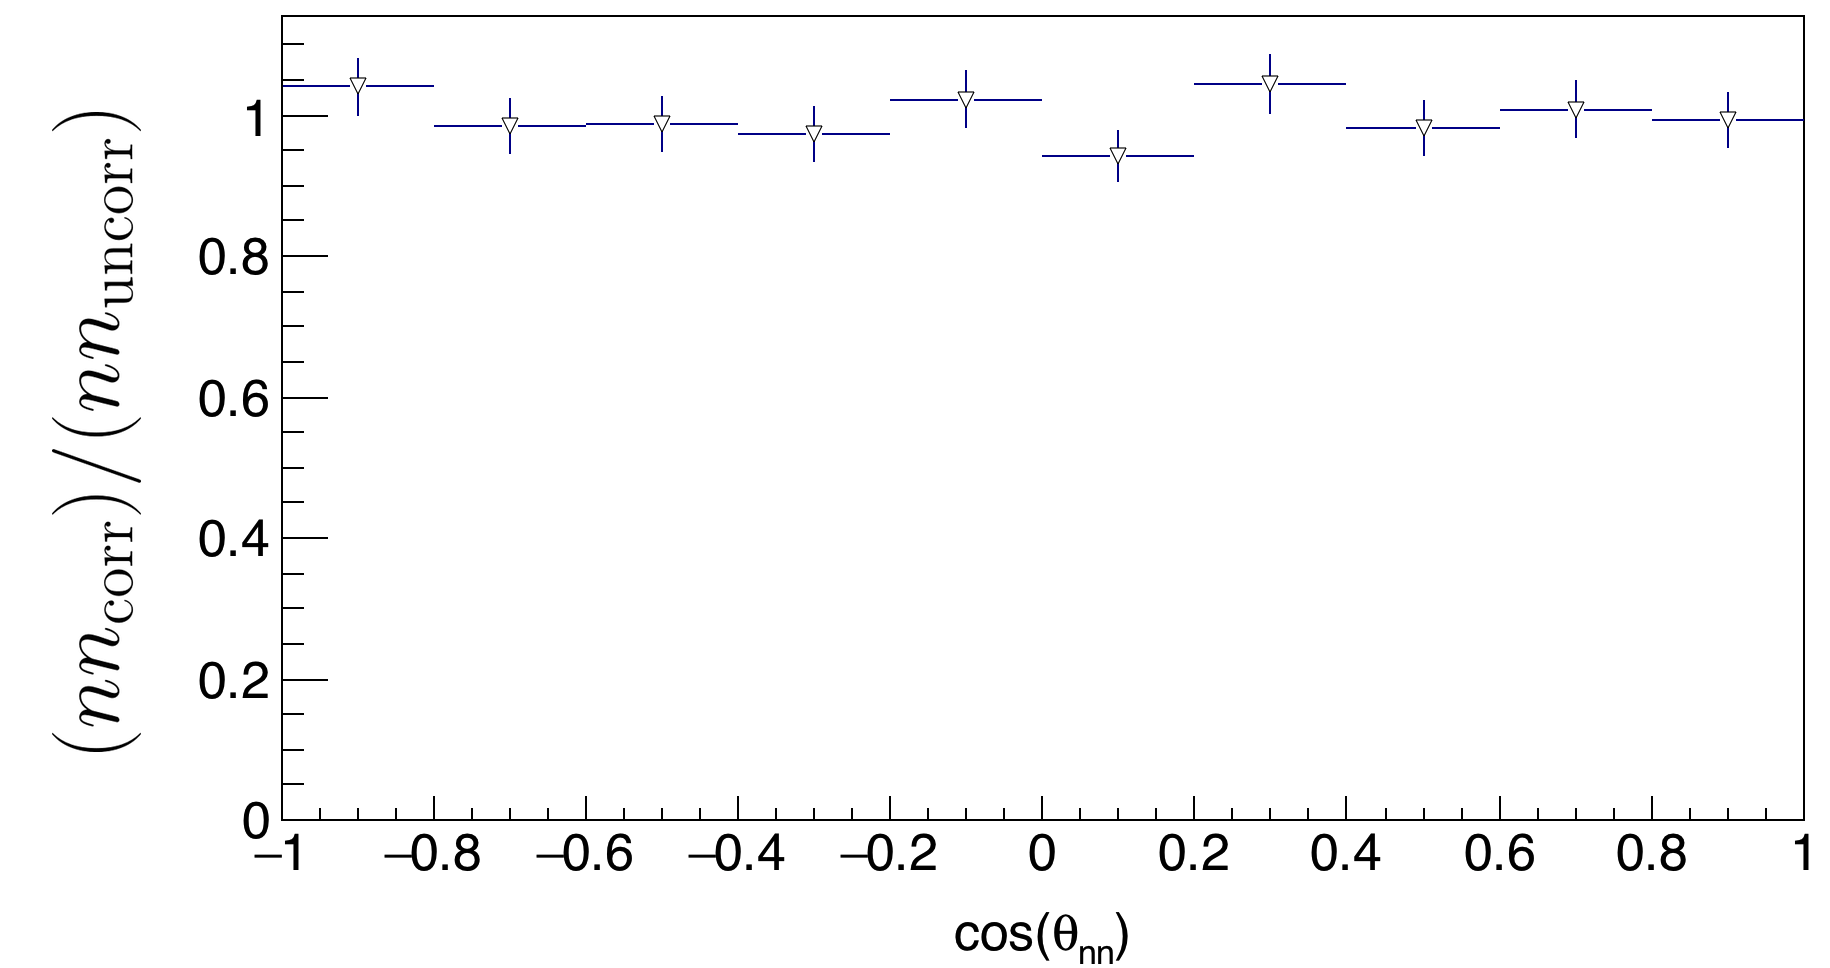
\includegraphics[width=0.9\textwidth]{Content/Methods/D2Otheta_nn.png}
\caption{The opening angle distribution of neutrons from the photo-disintegration of D$_{2}$O is uniform.
This is expected because the photo-disintegration of D$_{2}$O emits only a single neutron, and thus this distribution arises solely from neutron accidentals.}
\label{fig:D2Otheta_nn}
\end{figure}

\FloatBarrier
\subsection{Subtraction of Accidental Coincidences}
\label{Reconstruction of Accidental Coincidence}
The detection of two uncorrelated events in coincidence, whether caused by neutrons, photons, or noise, is referred to as an \emph{accidental}.
A small number of accidental photon events will exist in the neutron time of flight range because of the smearing of the photon peak.
These events are accidentals, because they are extremely likely to be due to photons from the beam, and not photons from fission.
There are also accidentals due to noise, which can be estimated with a non-neutron producing target made from aluminum (see Fig.~\ref{fig:Noise}).
The accelerator's current was adjusted so that there are, on average, less than 1.0 fissions per accelerator pulse, but nevertheless statistical fluctuations in the number of fissions per pulse result in accidental coincident neutrons that originated from different, and therefore, uncorrelated fissions.
There are also uncorrelated neutrons produced when multiple $(\gamma, n)$ reactions occur in a single pulse.
The $^{238}$U cross-section of $(\gamma, n)$, integrated over the relevant bremsstrahlung energy distribution, is about a factor of 5.5 times greater than it is for photofission (see Fig.~\ref{fig:CrossSection}).
As a result, it is unavoidable that there be a significant number of neutron coincidences caused by multiple $(\gamma, n)$ reactions relative to those caused by correlated fission neutrons.
If not subtracted from the result, the opening angle distribution of uncorrelated neutrons will wash out the signal from correlated neutrons. 
\begin{figure}[]
\centering
    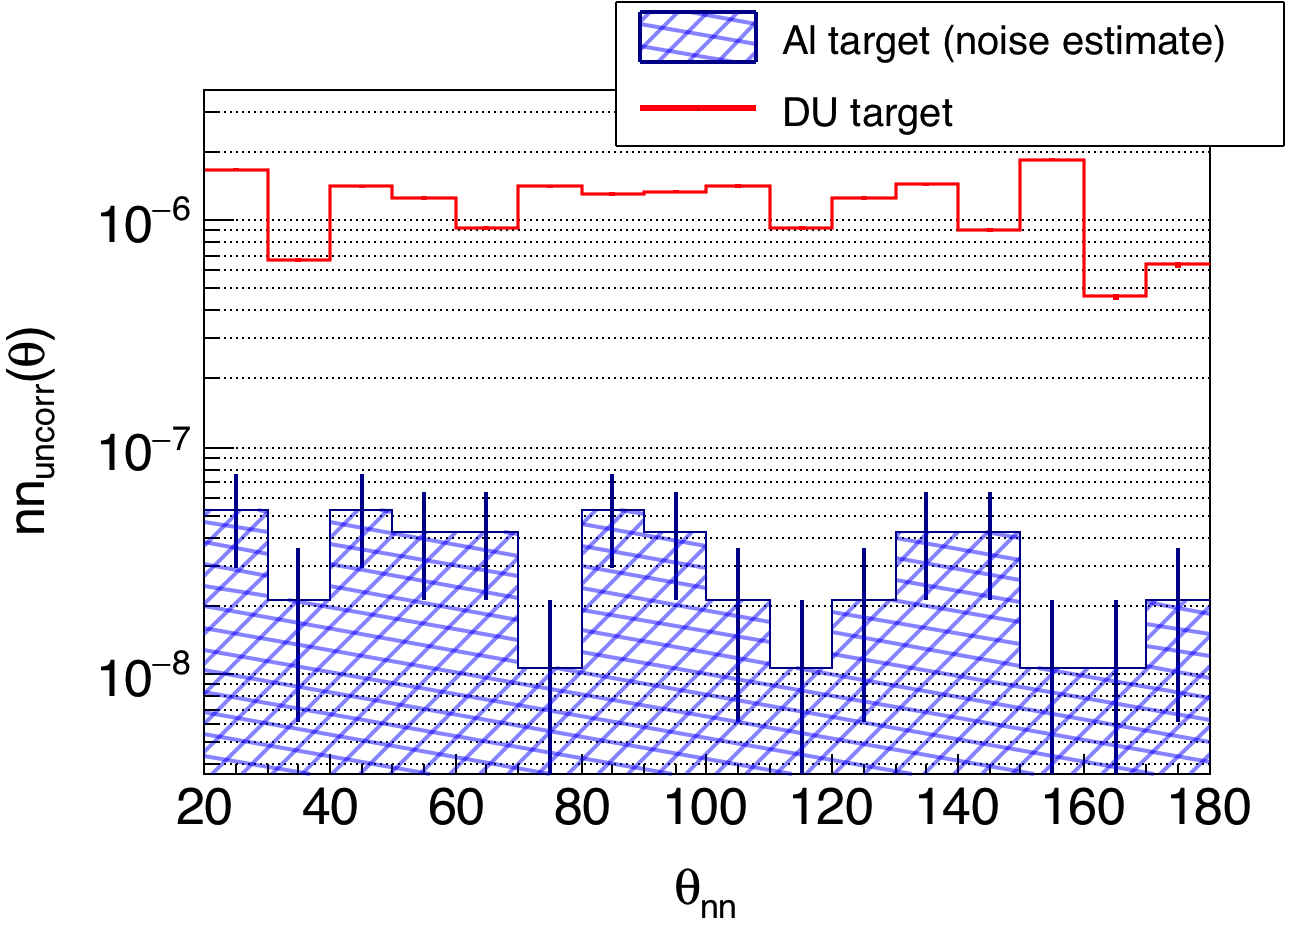
\includegraphics[width=0.8\textwidth]{Content/Methods/Noise.png}
    \caption{An Al target was designed to scatter the same number of photons as the DU target, thus serving as an equivalent non-neutron producing target well-suited to estimate noise.
    The rate of coincident events for the Al target is 3\% that of the DU target. 
        }
    \label{fig:Noise}
\end{figure}
\begin{figure}[]
\centering
    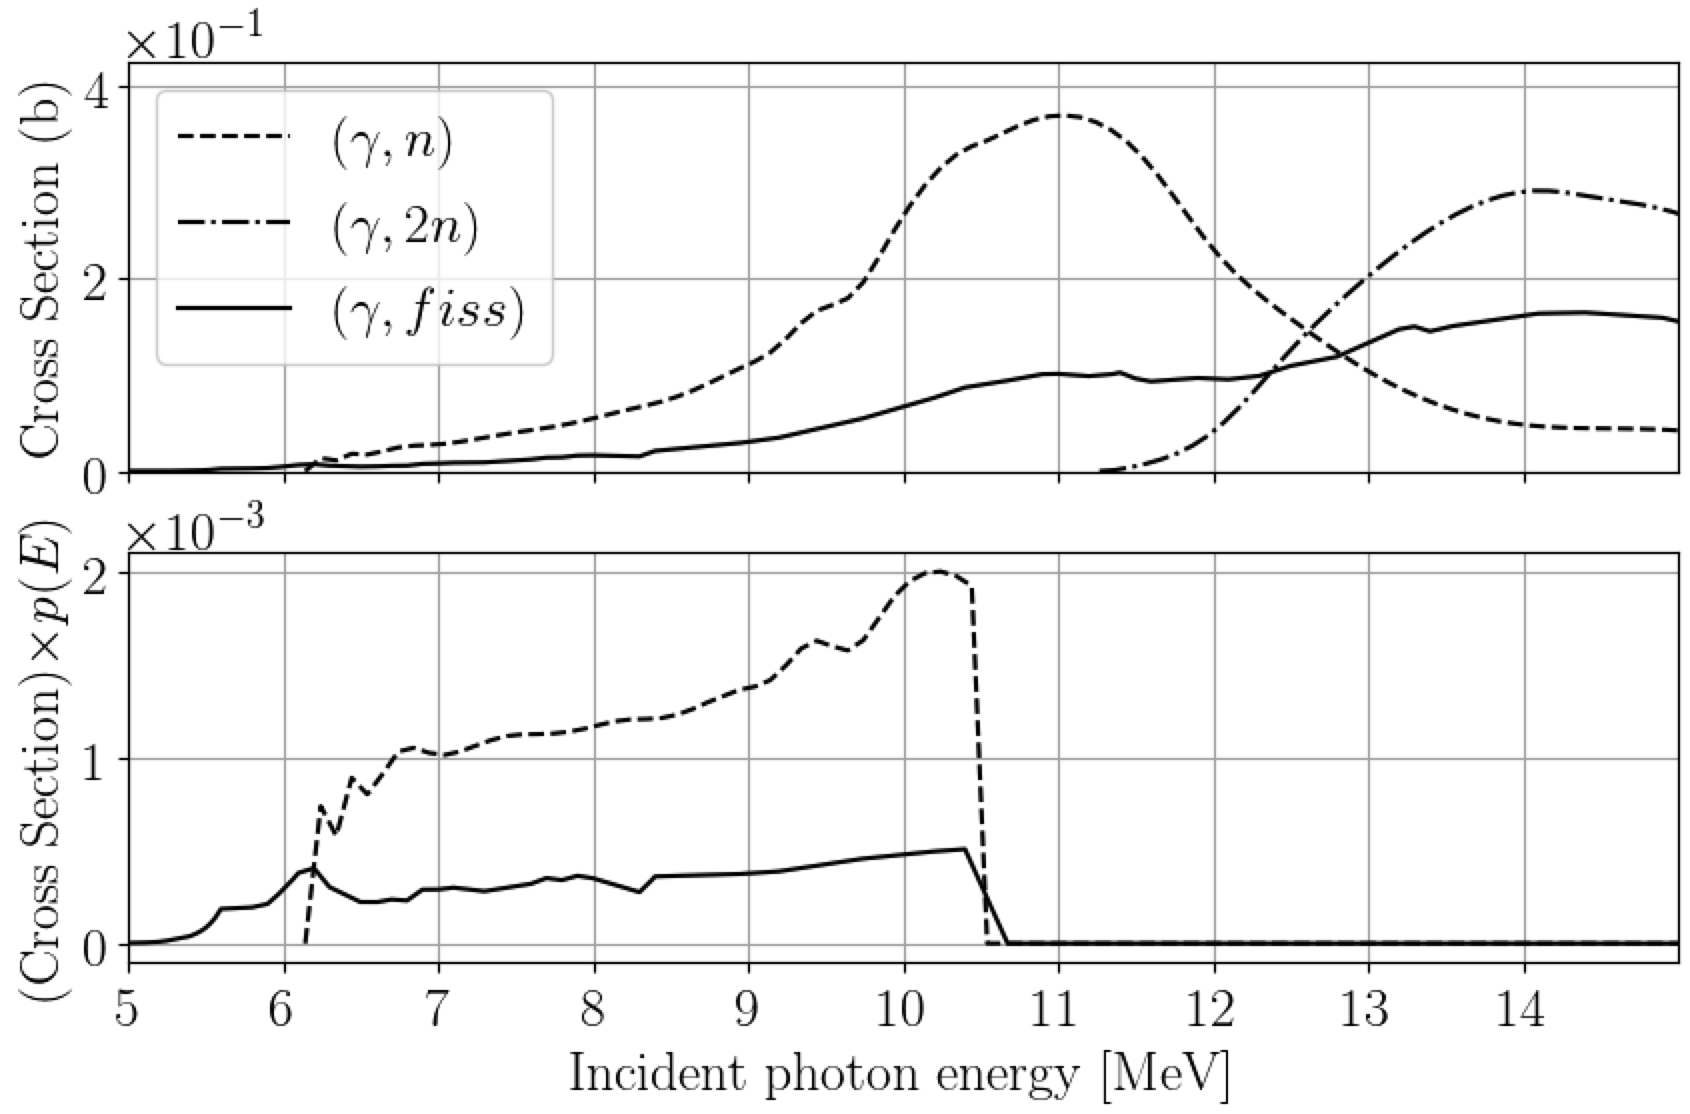
\includegraphics[width=0.95\textwidth]{Content/Methods/CrossSections.png}
    \caption{(top) ENDF cross-sections of $(\gamma$,fiss) and direct $(\gamma$,n) and direct $(\gamma$,2n).
    (bottom) Cross-sections integrated over the simulated relative rate of bremsstrahlung photons that reach the target as a function of photon energy. The integrated cross-sections of $(\gamma, n)$ is 5.5 times greater than for $(\gamma, \text{fiss})$. }
    \label{fig:CrossSection}
\end{figure}
\begin{figure}[]
\centering
    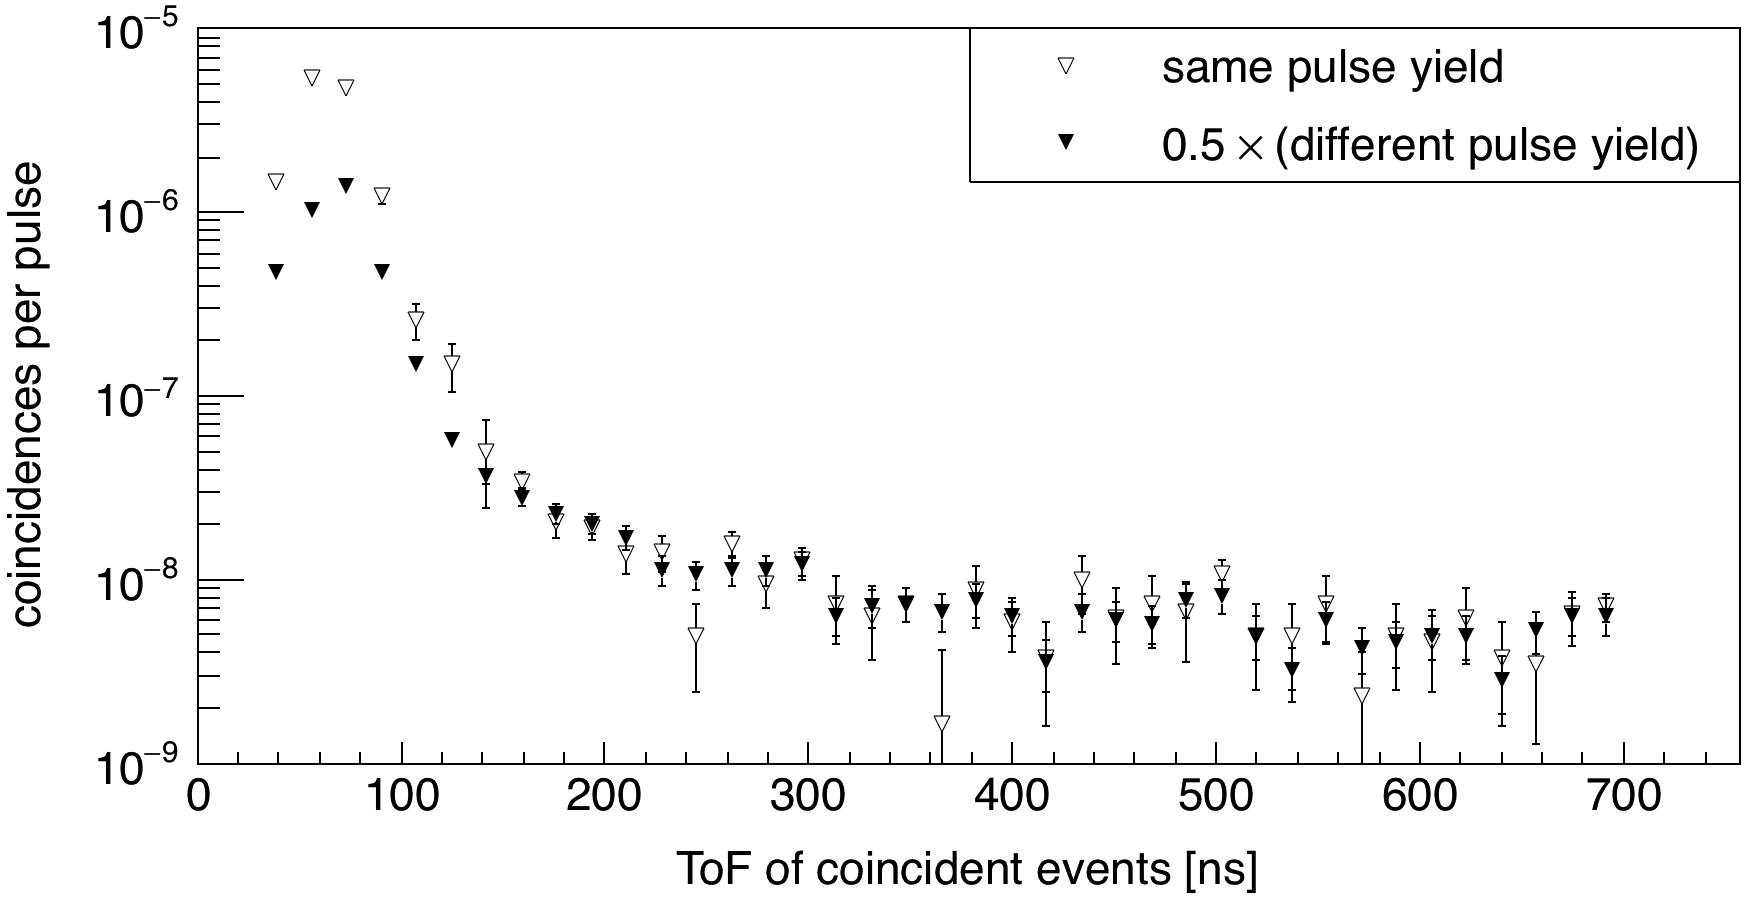
\includegraphics[width=0.9\textwidth]{Content/Methods/NoiseSubtraction.png}
    \caption{The different pulse yield captures the effects of noise due to accidentals.
    The y-axis represents the number of coincidences in which both events had a ToF within a given 20~ns wide bin.
    Because events with a ToF above 120~ns are predominately due to noise, which correspond to a 0.5 MeV neutron, the same pulse yield is equal to 1/2 times the different pulse yield.
    }
    \label{noise_siubtraction}
\end{figure}

The raw measurement consists of a mix of correlated and accidental neutron coincidences, that is
\begin{equation}
\label{eq:corr_uncorr}
nn_{\text{raw}}(\theta)= nn_{\text{corr}}(\theta) + nn_{\text{acc}}(\theta) \,
\end{equation}
where $nn_{\text{raw}}(\theta)$ and $nn_{\text{acc}}(\theta)$ are the rates, per pulse, of the detection of neutron pairs with opening angle of $\theta$ for all events and for accidental coincident events, respectively.

Because accidental coincidences consist of two independent events, it does not matter whether the two events occurred during the same pulse or during two different pulses, given that the two different pulses occurred at around the same time and thus under the same experimental conditions.
Thus, $nn_{\scaleto{DP}{4pt}}(\theta)$ is proportional to $nn_{\text{acc}}(\theta)$.
In other words,  $nn_{\scaleto{DP}{4pt}}(\theta)$ and $nn_{\text{acc}}(\theta)$ have opening angle distributions with the same shape.
However, $nn_{\text{acc}}(\theta)$ is not equal to $nn_{\scaleto{DP}{4pt}}(\theta)$, because there are, on average, twice as many events in a pulse-pair than there are in a single pulse.
For this reason, as the following analysis shows,~$nn_{\text{acc}}(\theta) = \frac{1}{2}nn_{\scaleto{DP}{4pt}}(\theta)$.

The number of uncorrelated events detected per pulse is assumed to follow the poissonian distribution, which describes the occurrence of independent random events.
Let $\lambda$ represent the mean number of uncorrelated events per pulse.
To determine the value of $\lambda$, one needs to know whether a given coincident event is in fact an accidental, as $\lambda$ only quantifies the rate of accidental coincidences.
Such information is not known, but the largest possible value for $\lambda$ is the mean number of events per pulse, because this assumes all events are uncorrelated.
This places an upper bound on $\lambda$ of $3\times 10^{-6}$ for this work, which is small enough to neglect all terms on the order of $\lambda^3$ or greater.

The per-pulse accidental coincidence rate of individual pulses summed over all opening angle bins, denoted by $\sum_{\theta} nn_{\text{acc}}(\theta)$, is equal to the poissonian probability of there being exactly two events detected in a single pulse\footnote{For the sake of brevity, cases of greater than two-fold coincidence are not considered in this analysis, and it is not necessary because of the low detection rates during this work.
It can be shown, however, that accounting for any number of coincidences, from zero all the way up to $\infty$-fold coincident events in a pulse or pulse-pair, will give the same answer.}:
\begin{equation} \label{math:SP}
    \begin{split}
    \sum_{\theta} nn_{\text{acc}}(\theta) & = \frac{e^{-\lambda}\lambda^{2}}{2!} \\
        &\approx \frac{\lambda^2}{{2}} + \mathcal{O}(\lambda^3) \, .
    \end{split}
\end{equation}
For the case of different-pulse pairs, a ``coincidence'' occurs when there is an event in both pulses.
Cases in which there are more than two events can be neglected due to their rare occurrence in this work.
Therefore, the per-pulse rate for different-pulse pairs, again summed over all opening angle bins, is the square of the poissonian probability of there being one event:
\begin{equation} \label{math:DP}
    \begin{split}
   \sum_{\theta} nn_{\scaleto{DP}{4pt}}(\theta)&= \left(e^{-\lambda}\lambda\right)^{2} \\
    &\approx \lambda^2 + \mathcal{O}(\lambda^3) \, .
    \end{split}
\end{equation}
For the reasons explained above, $nn_{\scaleto{DP}{4pt}}(\theta)$ and $nn_{\text{acc}}(\theta)$ have the same shape, thus, from Eq.'s (\ref{math:DP}) and (\ref{math:SP}) it follows that 
\begin{equation}
\label{eq:uncorr_DP}
nn_{\text{acc}}(\theta) = \frac{1}{2}nn_{\scaleto{DP}{4pt}}(\theta) \,.
\end{equation}

